\chapter{系统设计与架构}
本文在之前已详细介绍了用户语义理解模型的算法部分,为将算法与应用相结合,利用现有的跨界服务
网络系统JTangYdrail,设计了服务智能调用引擎的系统架构。本章将相对跨界服务
网络系统架构做简要介绍,之后展开讨论与语义理解相关的系统模块。

\section{跨界服务网络系统}
本文作者所在的课题组系统性地研究了跨界服务相关理论,并形成了跨界服务原型系统,
本节主要介绍系统整体架构以及跨界服务系统中两个核心模块服务交换机和服务路由器\cite{zheng2020service}。

  跨界服务系统是针对跨界服务运行时呈现高维异构、复杂动态、开放分布的特点,解决跨界服务网络管理中高效接入、安
  全交换、智能路由等关键技术,形成的跨界服务集成工程化方法,研制软硬件结合的跨
  界服务集成及运行支撑载体,包括跨界服务集成设计软件套件、服务交换机与路由器硬
  件环境。

  海量跨界服务分布于服务网络中,不同服务之间相互操作,通过服务交换及路由技术,实现跨界服务的查找、调用
  及跨界服务间的交互,同时利用基于认证授权的开放服务安全交换技术,保证交换
  过程中的数据安全。服务交换机和服务路由器是支撑载体的关键,采用软硬结合
  的设计方案来实现,如图\ref{fig:system}所示,服务交换机实现跨界服务的高效接入、访问控制、消
  息映射、认证授权等功能,实现域内企业服务的安全可靠的开放,其架构包括设施层(机
  柜、电源、接口等)、设备层(计算服务器、存储服务器)、网络层(虚拟路由器、虚拟
  防火墙)、应用层(服务接入、访问控制、服务缓存等)\cite{刘皇敏2019跨界服务网络关键技术研究}。服务路由器提供服务聚合、
  服务查找、服务路由等能力,把异构服务联成网络,是跨界服务互联的基础设施,其架
  构包括设施层(机柜、电源、接口等)、设备层(计算服务器、存储服务器)、网络层(状
  态感知、消息路由等功能)、应用层(服务索引、服务查找、服务路由等)。

  \begin{figure}[htbp]
    \centering
    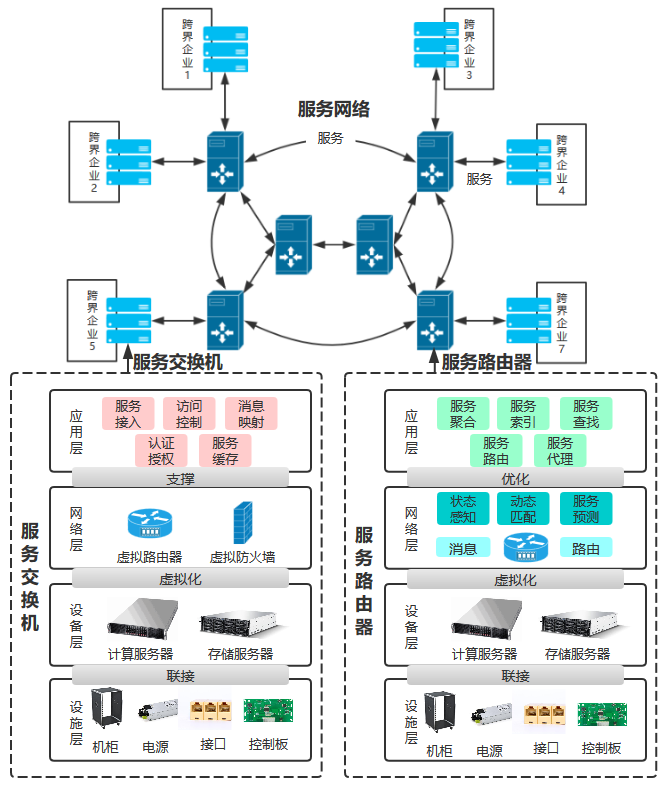
\includegraphics[width=10cm]{./images/system.png}
    \caption{JTangYdrail系统架构\cite{zhanghuan}}
    \label{fig:system}
  \end{figure}

  服务交换机是跨界服务网络上最下层节点,
  使用服务地址在交换层接收并转发服务相关的数据,与实际服务直接相关,
  是服务的拥有者以及一次服务远程调用的发起者。
    服务路由器是在服务网络中转发服务元信息的网络设备,一方面,服务路由器从服务交换机收集服务信息,并在整个网络中广播数据。 
    另一方面,如果用户调用服务,则服务路由器会将请求转发到相应的服务节点。 
    % 如图\ref{fig:switchboard}所示,主要包含以下几个模块:

% 1)注册模块:维护企业的服务信息和业务数据,
% 服务成功注册后,服务信息将存储在本地,并且其元数据将通过泛洪或其他方式广播到整个网络。
% 此后不久,其他服务交换机即可搜索和使用该服务交换机上服务。

% 2)适配器模块:旨在支持环境异构,AdM提供了各种适配器,可以通过不同的语言实现这些适配器,以实现与异构服务的通信。
% 在语义上兼容前提下,尽管硬件和软件平台,语言和API不同,但连接到不同适配器的各种服务在跨界服务系统仍将被连接和集成。

% 3)策略模块:使用多种策略来提高性能,代理策略使用户可以通过代理调用服务,服务交换机的负载平衡策略通过增加进程数来实现可伸缩性和负载平衡,
% 服务缓存策略使某些节点可以缓存服务调用的结果,从而可以充分利用网络中边缘节点的资源。 

% 4)映射模块:旨在为用户带来便利,以特定格式调用服务或接收结果。
%  提供了直观的图形界面,供用户生成规则文件。 
 
% 5)权限模块:是基于密钥加密技术设计的,并使用基于角色的访问控制策略来保护数据的安全性。

  % \begin{figure}[htbp]
  %   \subfloat[JTangYdrail 服务交换机软件架构\cite{zhanghuan}]{
  %     \centering
  %     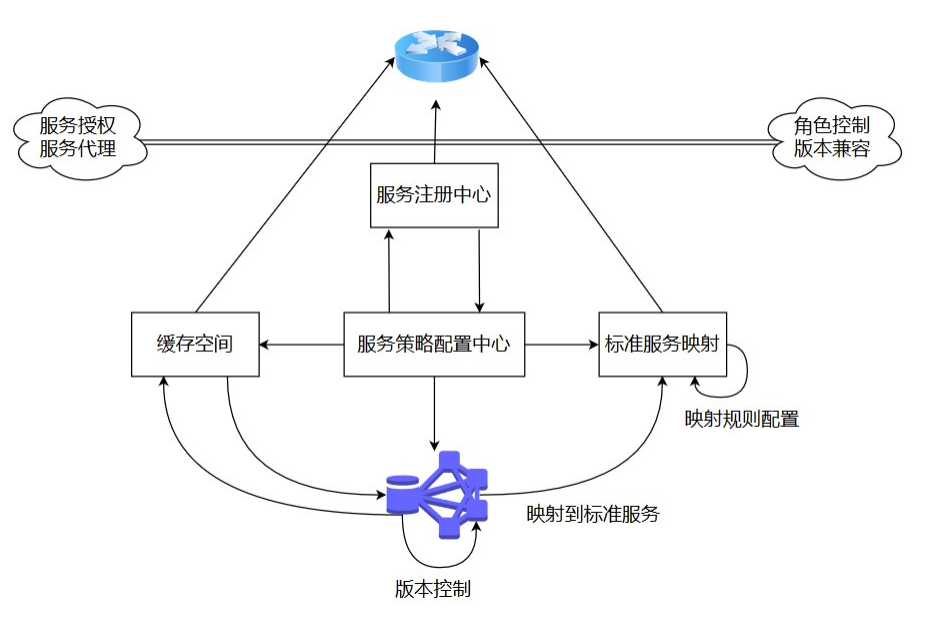
\includegraphics[width=8cm]{./images/switchboard.png}
  %     \label{fig:switchboard}
  %   }
  %   \subfloat[JTangYdrail 服务路由器软件架构\cite{zhanghuan}]{
  %     \centering
  %     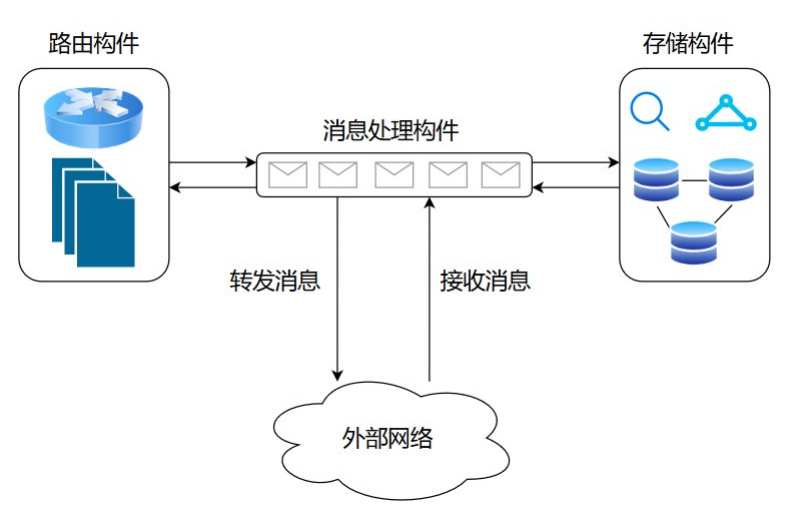
\includegraphics[width=8cm]{./images/router.png}
  %     \label{fig:router}
  %   }
  %   \caption{服务交换机和服务路由器架构}
  %   \label{fig:switchboardAndRouter}
  %   \end{figure}
    
    % 服务路由器的结构如图\ref{fig:router}所示,其中包含路由组件,存储组件,处理器组件等:

    % 1)存储模块:由三部分组成:服务缓存,包括一些服务元数据和一些查询结果;
    % 路由信息,这是整个网络的基础,以及服务网络的结构信息。
    
    % 2)路由模块:功能是根据服务ID转发服务请求,该服务ID与传统网络中的IP地址完全不同。
    
    % 3)处理器模块:提供内部和外部资源之间的通信机制。消息有两种类型:服务消息和路由消息。
    % 一旦收到消息,它将由PrC进行预处理,然后传输到路由组件或存储组件。
    
    % 4)标准服务模块:标准化服务组件设计用于服务网络中功能相似的同类服务,
    % 当发现Web服务的任何故障时,它可以通过使用标准化服务动态地将服务替换为合适的服务,从而大大提高了服务的可用性和可靠性。


  
  
  
\section{智能服务调用引擎}

上一节介绍了跨界服务网络系统,是本文主要依托的平台,随着系统的运行平台内部的服务由于不断接入会累积增多,
对于大型跨界服务网络,服务数量会非常庞大。
用户在进入系统后面对如此量级的服务,在服务检索时无法快速定位到自己想要的服务,需要花费大量成本,
因此如何提升用户检索服务时的体验成为问题。借助对话系统的思想,本节在系统中提出了以语义理解模块为核心的智能服务调用引擎,
用户进入相应前端以后,可以输入带有自己意图的语句传给后台暴露的接口,智能服务调用引擎接受语句以后进行语义理解,
识别并找出系统内部与之匹配的服务,从句子中提取参数完成调用返回结果,从而解决了用户检索服务困难的问题,
简化了用户操作,提升了用户体验,让系统更加智能化。

在跨界服务网络中,所有的服务都部署在服务交换机上,因此智能服务调用引擎也运行在服务交换机系统内。
引擎集成在服务交换机系统内运行在跨界服务网络中,因此智能调用的能力是在后端的,与用户使用的终端系统解耦,最终在服务端暴露智能调用的接口供
跨界服务网络的使用者选择。

\begin{figure}[htbp]
  \centering
  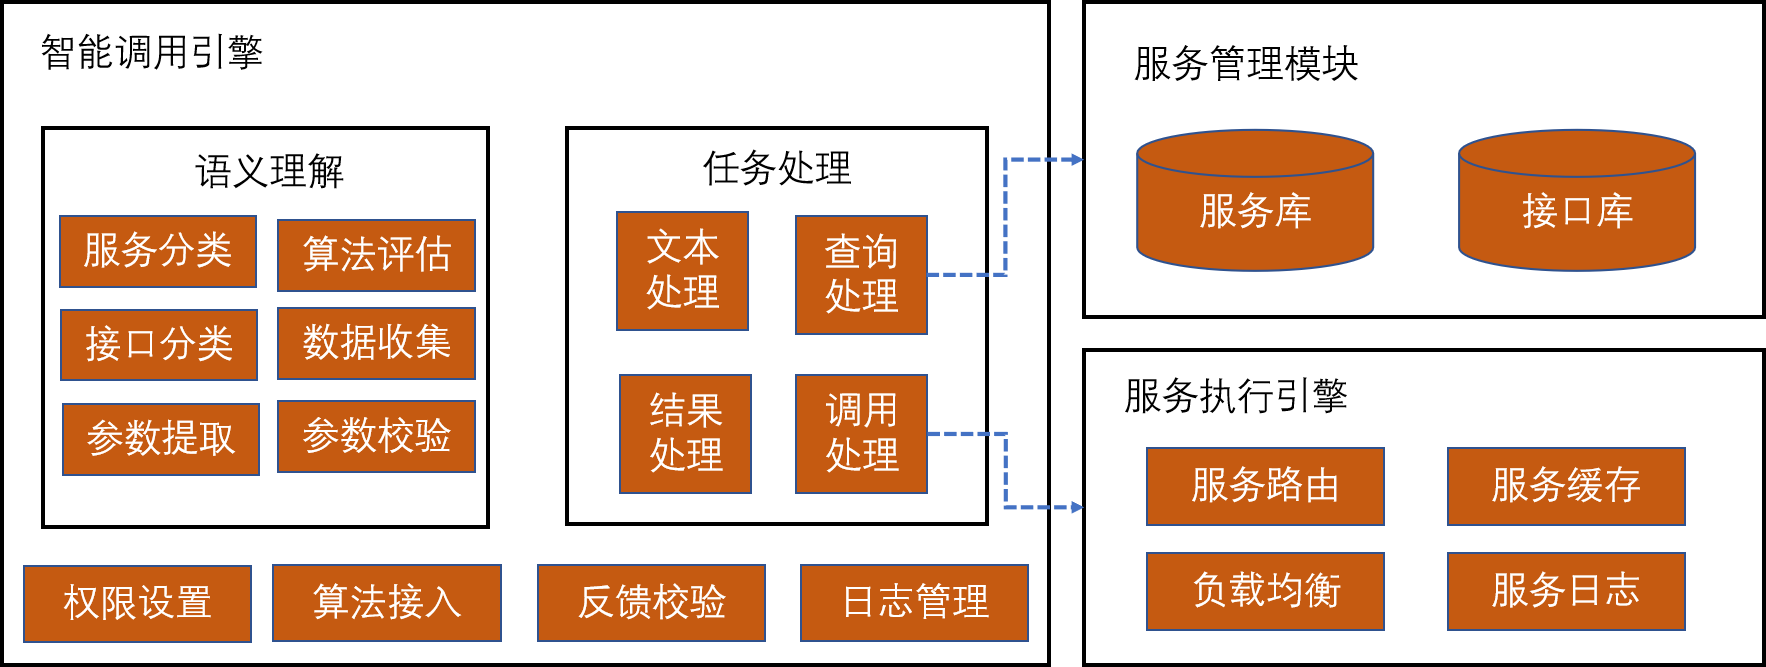
\includegraphics[width=15cm]{./images/yinqing.png}
  \caption{服务智能调用引擎架构}
  \label{fig:yinqing}
\end{figure}

如图\ref{fig:yinqing}所示,智能服务调用引擎可以抽象为语义理解和任务调度两个模块:

(1)语义理解:核心任务是本文一直在讨论的三项任务服务分类、接口分类和参数填充,接收的是用户输入的一句有目的性的话,识别用户的意图,根据
用户意图匹配相应的服务以及匹配该服务要执行的操作,找到匹配的服务以后,从用户输入的语句中提取在服务执行前需要
的执行参数,该模块算法采用的是实验性能最优的BERT-co-interactive模型。此外我们增加了数据收集模块,在每次调用之后,引擎会自动收集本次输入的语句作为数据保存,
以此来丰富平台的数据集,同时我们计划定期人工评估算法准确率进而优化模型。

(2)任务调度:该模块主要是智能调用需要解决的工程问题,使引擎能与跨界服务网络系统结合。文本处理器主要做了边界字符和停用词过滤处理,处理好的语句传入模型输入层,模型识别
出本次服务调用需要的服务、接口和参数信息后,会首先通过查询处理器向系统中服务管理模块按关键字查询得到被调用服务在系统中的执行逻辑,这里会有一个校验逻辑,校验
内容包括调用者的权限合法性以及参数信息是否有误等,校验通过以后,调用处理器会带着必要的各项参数向服务执行引擎发送请求,在跨界服务网络中找到服务源完成本次
服务的调用并返回结果到结果处理器,经结果处理器封装的最终结果会返回给用户。

如图\ref{fig:yinqinliucheng}所示,描述了智能服务调用引擎运行流程,流程大致可分为三个部分:

第一部分是交互模块。交互模块主要将用户传来的语句进行预处理传入智能解析模块,同时将系统执行服务调用
后的结果进行封装返回给前台调用者。

第二部分是智能问答模块。这其中主要逻辑就是本文重点研究的语义理解算法,包括服务分类、接口分类和参数提取,同时
也包含了必要的服务调用权限校验、参数校验和对话管理等逻辑。

\begin{figure}[htbp]
  \centering
  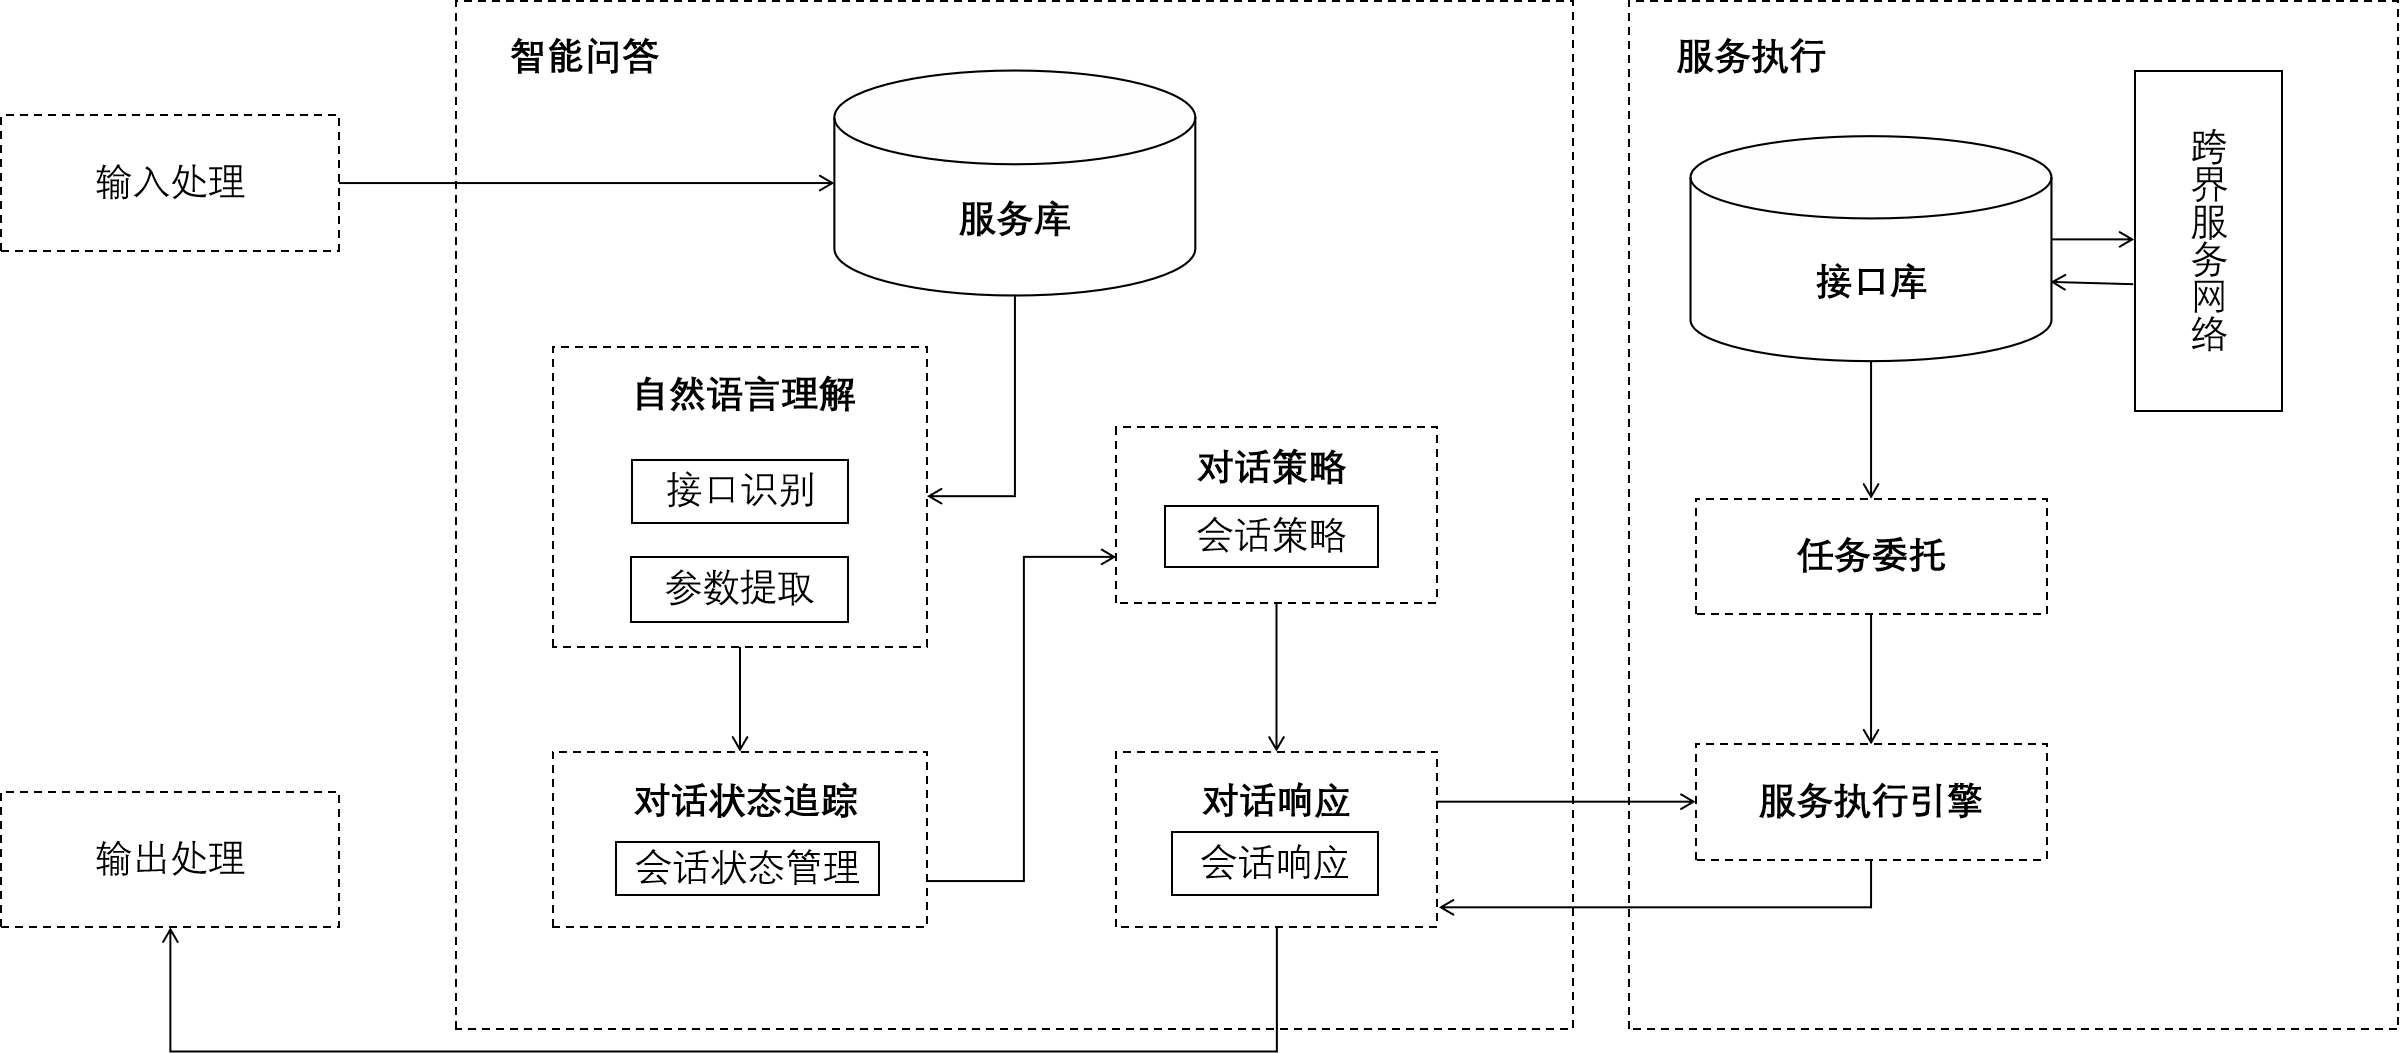
\includegraphics[width=15cm]{./images/yinqinliucheng.png}
  \caption{智能服务调用引擎运行流程}
  \label{fig:yinqinliucheng}
\end{figure}

第三部分是服务执行模块。该模块根据解析用户意图以后得到的信息在跨界服务网络中查询到相应服务的位置,完成服务调用后
返回执行结果到输入输出模块。

\subsection{交互模块}
交互模块是与前台距离最近的一层,因此需要在后端暴露相应的接口供前端调用。在课题组已有的JTangYdrail系统中,后端采用java语言springboot框架实现,因此
交互模块使用相同的方式,至于用户实际使用的前台产品,可以是网页或者客户端,这与跨界服务网络本身解耦。

以http请求为例,用户在前端输入带有意图的语句通过http传入交互模块的后台接口,解析出数据以后得到用户语句,
首先会进行用户权限的校验以及安全信息(如token等)的校验以验明用户身份和权限。
然后会进入输入处理模块进行文本预处理。
文本的预处理特别重要,如果句子中包含了太多无关词(这些词被称作停用词),算法性能会受影响,因此本文
在文本预处理时引用了停用词过滤。比较常见的中文停用词如“的”、“在”以及语气词等,他们的存在对语义理解没有贡献,相反如果分词工具使用他们错误的分词,
会降低模型准确率,本文利用网上已有的中文停用词词典在结巴分词工具处理前对用户语句做了停用词过滤。处理好之后的用户语句被传入智能解析模块进行语义理解分析。

在后台系统完成服务智能调用以后,交互模块会对本次服务调用进行postprocess,包括异常处理和数据封装等。异常的产生是由于跨界服务网络环境在不断动态变化,
上传在服务交换机的服务可能由于内部原因变得无法使用,同时节点信息在网络中更新有延迟,因此引擎可能检索出已不存在的服务从而产生服务调用异常,除此之外,
网路中服务路由器连接不可达导致服务调用请求无法被接受等原因也可能导致异常。如若服务成功调用并返回,由于服务种类众多返回结果的数据类型也是形态各异,
因此需要交互模块做统一的数据封装对外返回httpResponse结果。

\subsection{智能问答}
智能问答是智能服务调用引擎的核心,解决的是任务型对话系统的核心诉求,即识别用户的意图,根据
用户意图匹配相应的服务以及匹配该服务要执行的操作,找到匹配的服务以后,从用户输入的语句中提取在服务执行前需要
的执行参数,此模块由以下几个小模块组成:

(1)服务库。
服务库、接口库是智能服务调用引擎为语义理解相关的服务和接口独立建立的索引库,与系统中原有的服务数据库独立,它省略了系统中原有的服务数据库
其他无关的字段(如创建时间,创建人等),只保留与服务调用相关的字段,目的是为了加速索引过程和节省引擎占用的空间。
本文筛选了跨界服务网络系统中用户使用较多的几类服务的语料信息,包括“航班flight”,“音乐music”,
“天气weather”,“火车train”,“地图map”,“股票stock”,“医疗medical”,“新闻news”共八大类服务用于实验,
这些信息使用mysql数据库表进行保存。
再根据这些服务的接口构建接口类别的全集,例如“query”,“play”,“order”等,本文为每一类服务构建了接口库,
确定了服务接口以后,服务接口调用时的参数(语义槽)也就确定了,如“songName”,“singer”,“startCity”,“endCity”等,本文为每一个接口构建了参数库。
智能服务调用引擎中包含了服务、接口和参数信息的服务库主要用于快速索引和校验。

(2)语义理解。 
语义理解是整个智能解析部分的核心,系统接收的是用户输入的一句有目的性的话,在语义理解的过程中,
首先要识别用户的意图,根据
用户意图在系统中匹配相应的服务以及匹配该服务要执行的操作;之后,对于在服务执行前
必要的执行参数,需要从用户输入的语句中提取,这三项任务是语义理解的主要工作。
当前中文语义理解任务有着诸多挑战,如特定下游任务缺乏充分的数据集,用户表述意图模糊、随意不规范,一词多义等,为此我们利用
前面章节提出的BERT-co-interactive模型来完成语义理解工作,
以调用火车信息查询服务为例,
用户在进入跨界服务网络系统后,传入“查询成都前往杭州的火车票”,
模型将识别出该语义对应系统内部的<train服务>,接口类型为<query查询>,语义槽(即服务参数)为<startCity起始地>成都和<endCity目的地>杭州。

(3)对话管理。
对话管理模块主要用于保障用户对话过程的鲁棒性,主要包括对话状态追踪、对话策略和响应。
对话状态$S_{t}$指截至t时刻,用户向系统提供的语句信息以及系统掌握的用户身份信息等所有信息抽象化后得到的数据结构,
对话策略是根据用户当前的对话状态$S_{t}$选择最佳执行动作让人机对话顺利进行,帮助用户达到服务调用的目的。
举例来说,用户传入后台的语句为“查询到北京的机票价格”,此刻的对话状态$S_{t}$可由语义理解模块的输出、用户历史信息以及用户基本信息构成,
对话管理模块下一步的响应动作可能有以下几种:

a)询问缺省参数,如“请问是从哪里出发”;

b)向用户确认参数,如“请问是从您所在地出发吗”;

c)直接将信息传入下一模块,进行服务调用。

由此可见对话管理模块通过对用户对话状态的分析产生相应的对话策略并对之做出响应。

\subsection{服务执行}
服务执行模块是智能服务调用引擎的执行逻辑,智能问答模块产生的响应如果是服务调用,就会带着必要的参数向服务执行模块发送请求。
跨界服务网络中的服务通常为远程调用,这是因为用户连接请求的交换机中可能不存在本次服务调用需要的服务,因此需要交换机通过
路由器的路由功能找到服务在跨界服务网络中的真实地址,最终完成远程的服务调用。
由于跨界服务网络环境在不断动态变化,
上传在服务交换机的服务可能由于内部原因变得无法使用,同时节点信息在网络中更新有延迟,因此引擎可能检索出已不存在的服务从而产生服务调用异常,
所以服务执行模块包含了异常处理逻辑。
在完成了服务调用了以后,该模块会将调用结果返回给交互模块。


\section{原型系统展示}
在跨界服务理论基础上,实现了跨界服务网络平台的原型系统,系统被命名为JTangYdrail(图\ref{fig:logo})。
跨界服务网络与支撑载体系统依托于课题《跨界服务集成方法与支撑载体》,包含跨界服务交换机子系统、跨界服务路由器子系统和
跨界服务网络子系统。通过跨界服务交换机子系统,可以实现企业服务的包装、开放、部署和管理,并提供相关原生工具;通过跨界服务路由器
子系统,可以实现服务路由器的管理与可视化监控,实时掌握当前路由器的运行情况;通过跨界网络子系统,可以实现对全局
所有自网络及其关联的服务交换机和服务路由器的动态监控,并可对子网络进行管理。

\begin{figure}[htbp]
  \subfloat[JTangYdrail 首页]{
    \centering
    
\includegraphics[width=8cm]{./images/ketisan.png}
    \label{fig:ketisan}
  }
  \subfloat[JTangYdrail logo]{
    \centering
  
\includegraphics[width=8cm]{./images/jianmu.jpg}
  \label{fig:logo}
  }
  \caption{JTangYdrail总览}
  \end{figure}
  如图所示,JTangYdrail系统主要包含服务交换机管理、服务交换机工具和服务智能调用三个模块\ref{fig:sangemokuai}。
  服务交换机管理模块是系统的核心部分,主要包括服务管理,流程管理,申请管理和用户管理等功能,管理跨界服务网络中与服务相关
  的所有信息;服务交换机工具工具模块包括标注服务映射,物联网服务,服务包装等功能,这些功能均以工具形式嵌入JTangYdrail系统,
  是系统的附加能力;服务智能调用是与本文相关的模块,在跨界服务网络中暴露智能调用的能力,对用户输入的语句识别后智能执行相应的服务。

  \begin{figure}[htbp]
    \centering
    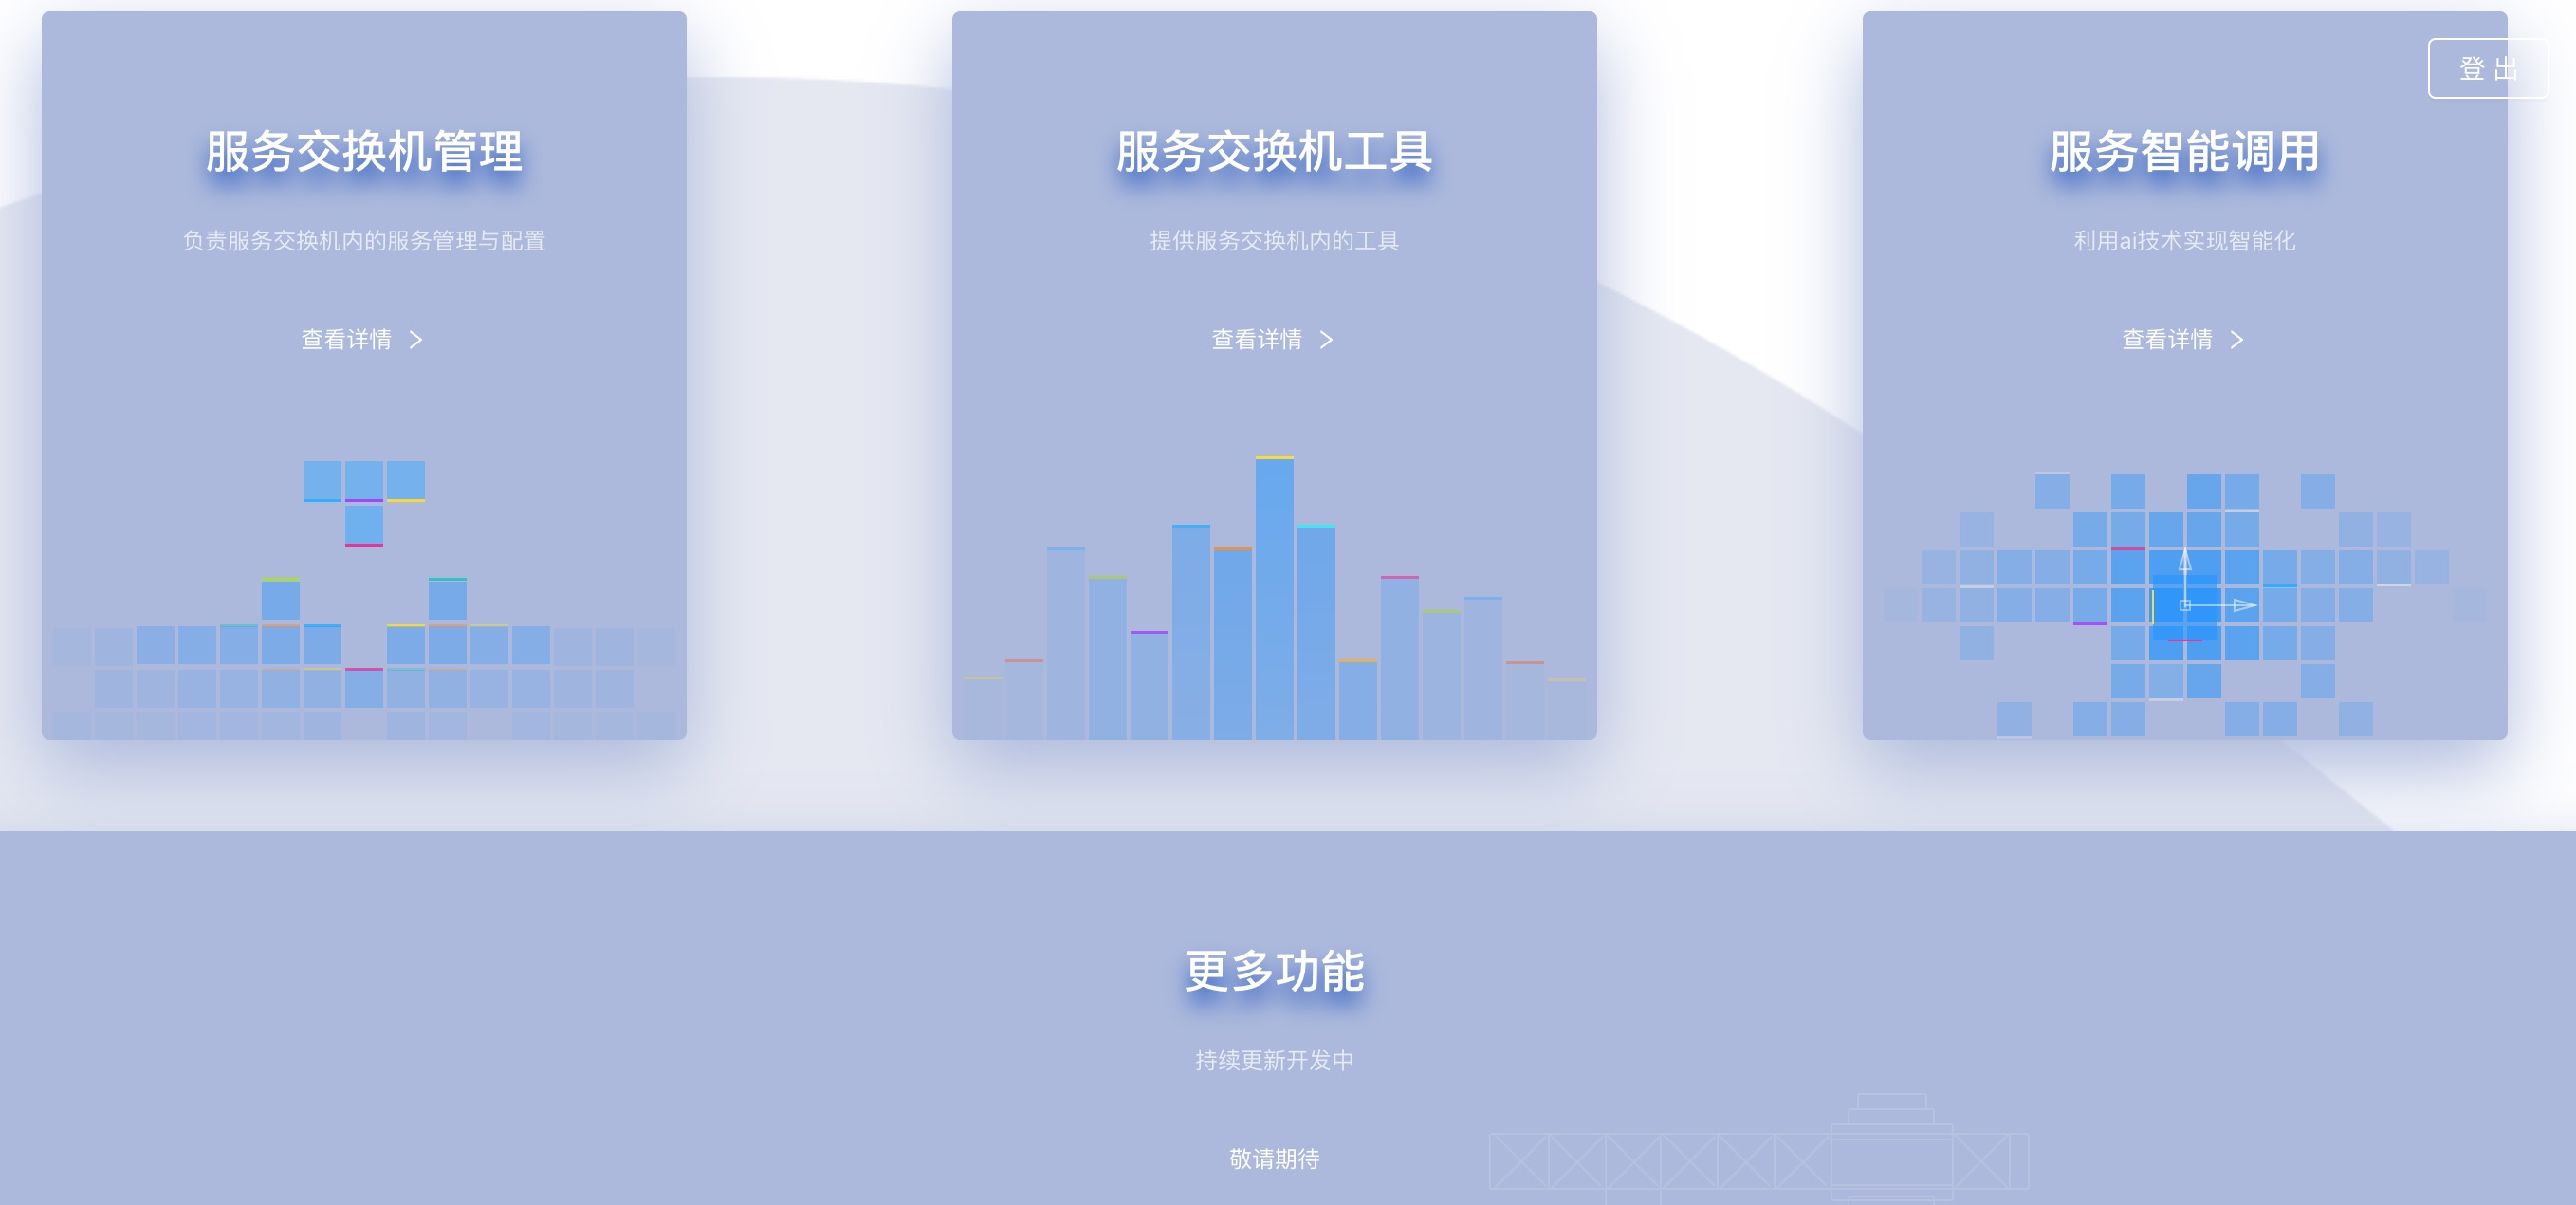
\includegraphics[width=17cm]{./images/sangemokuai.png}
    \caption{JTangYdrail 主要模块}
    \label{fig:sangemokuai}
  \end{figure}

本模块是系统的核心部分,进入系统后,点击服务详情页面对服务做CRUD,mapping,api management,test等一系列相关管理操作,
以及查看服务API的interface信息,parameter信息和SDK信息等。

如图\ref{fig:fuwuguanli}为服务管理模块的展示,服务管理的主要功能为: 
总览当前交换机内部所有服务的信息和实现对服务的增删改以及设置服务启用状态,
流程管理的主要功能为总览当前交换机内部所有流程的信息和实现对流程的增删改以及设置流程状态,
服务申请管理主要包含
企业对外进行服务申请需要的界面,可以申请其他服务交换机上的服务并实时反馈对方的审核信息,
部门管理的主要功能为
管理服务交换机中的各个部门,包括对部门信息的增删改查以及查看挂载在部门下的服务,
外部服务审批管理的主要功能为审核外部服务申请。
\begin{figure}[htbp]
  \subfloat[服务管理]{
    \centering
    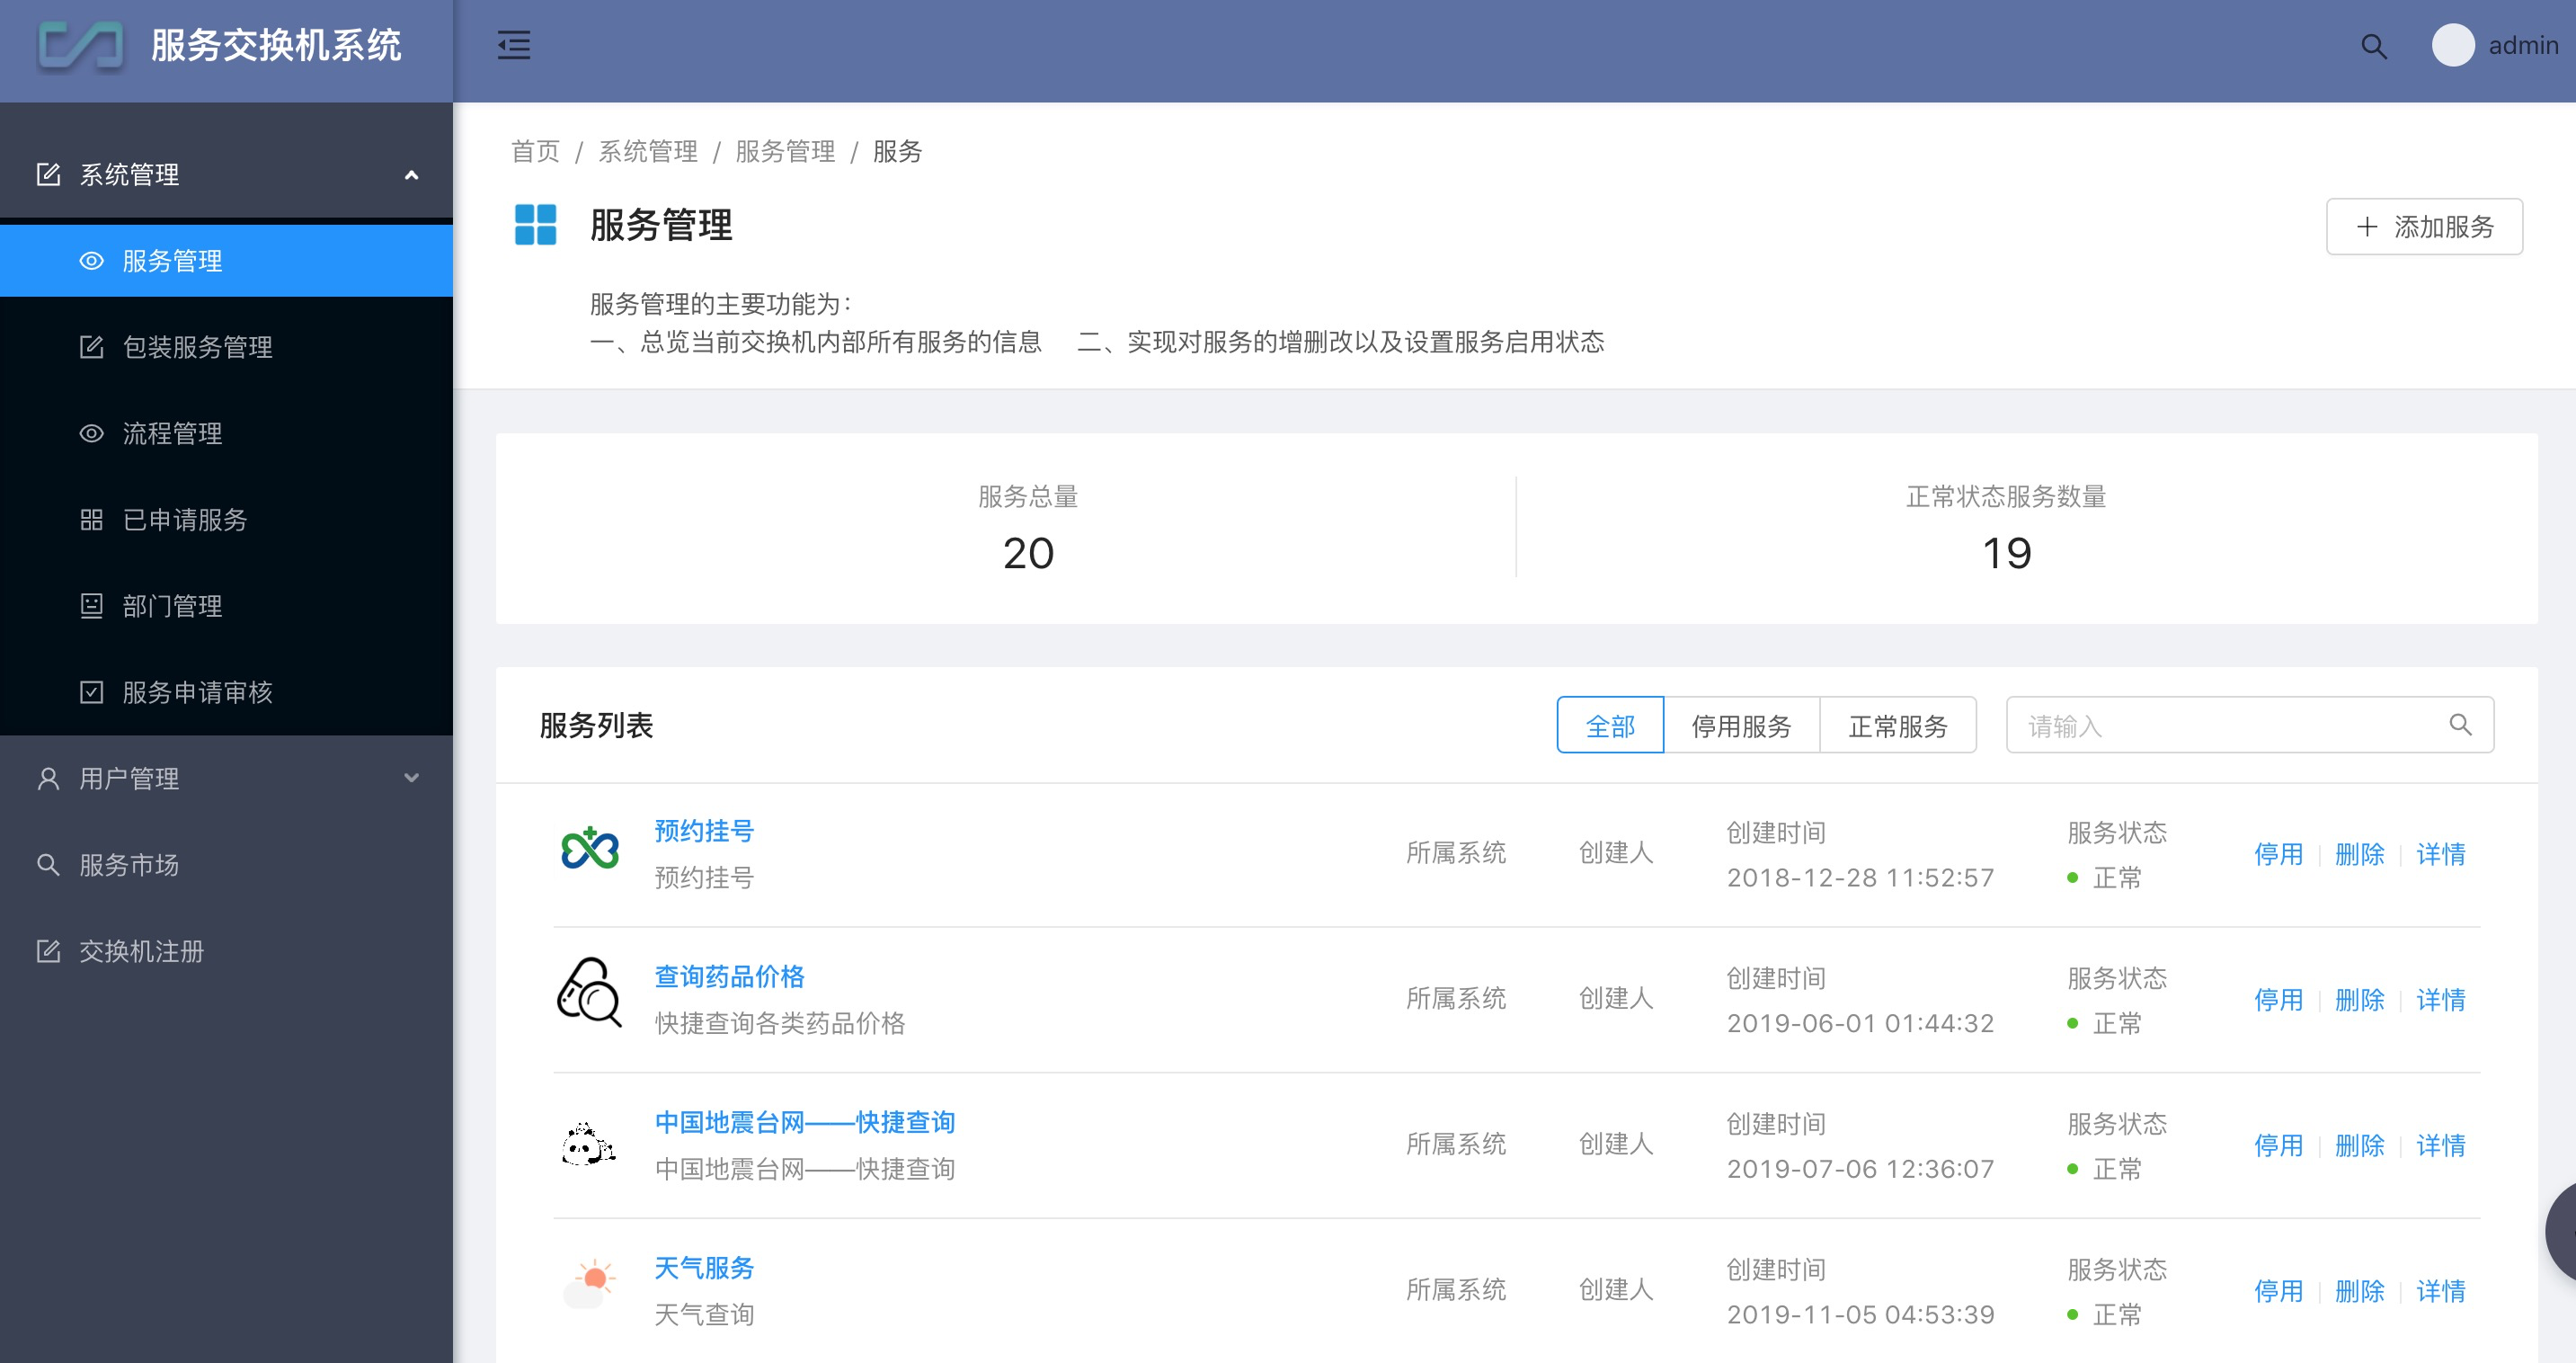
\includegraphics[width=8.3cm]{./images/fuwuguanli1.png}
    \label{fig:fuwuguanli1}
  }
  \subfloat[服务详情]{
    \centering
  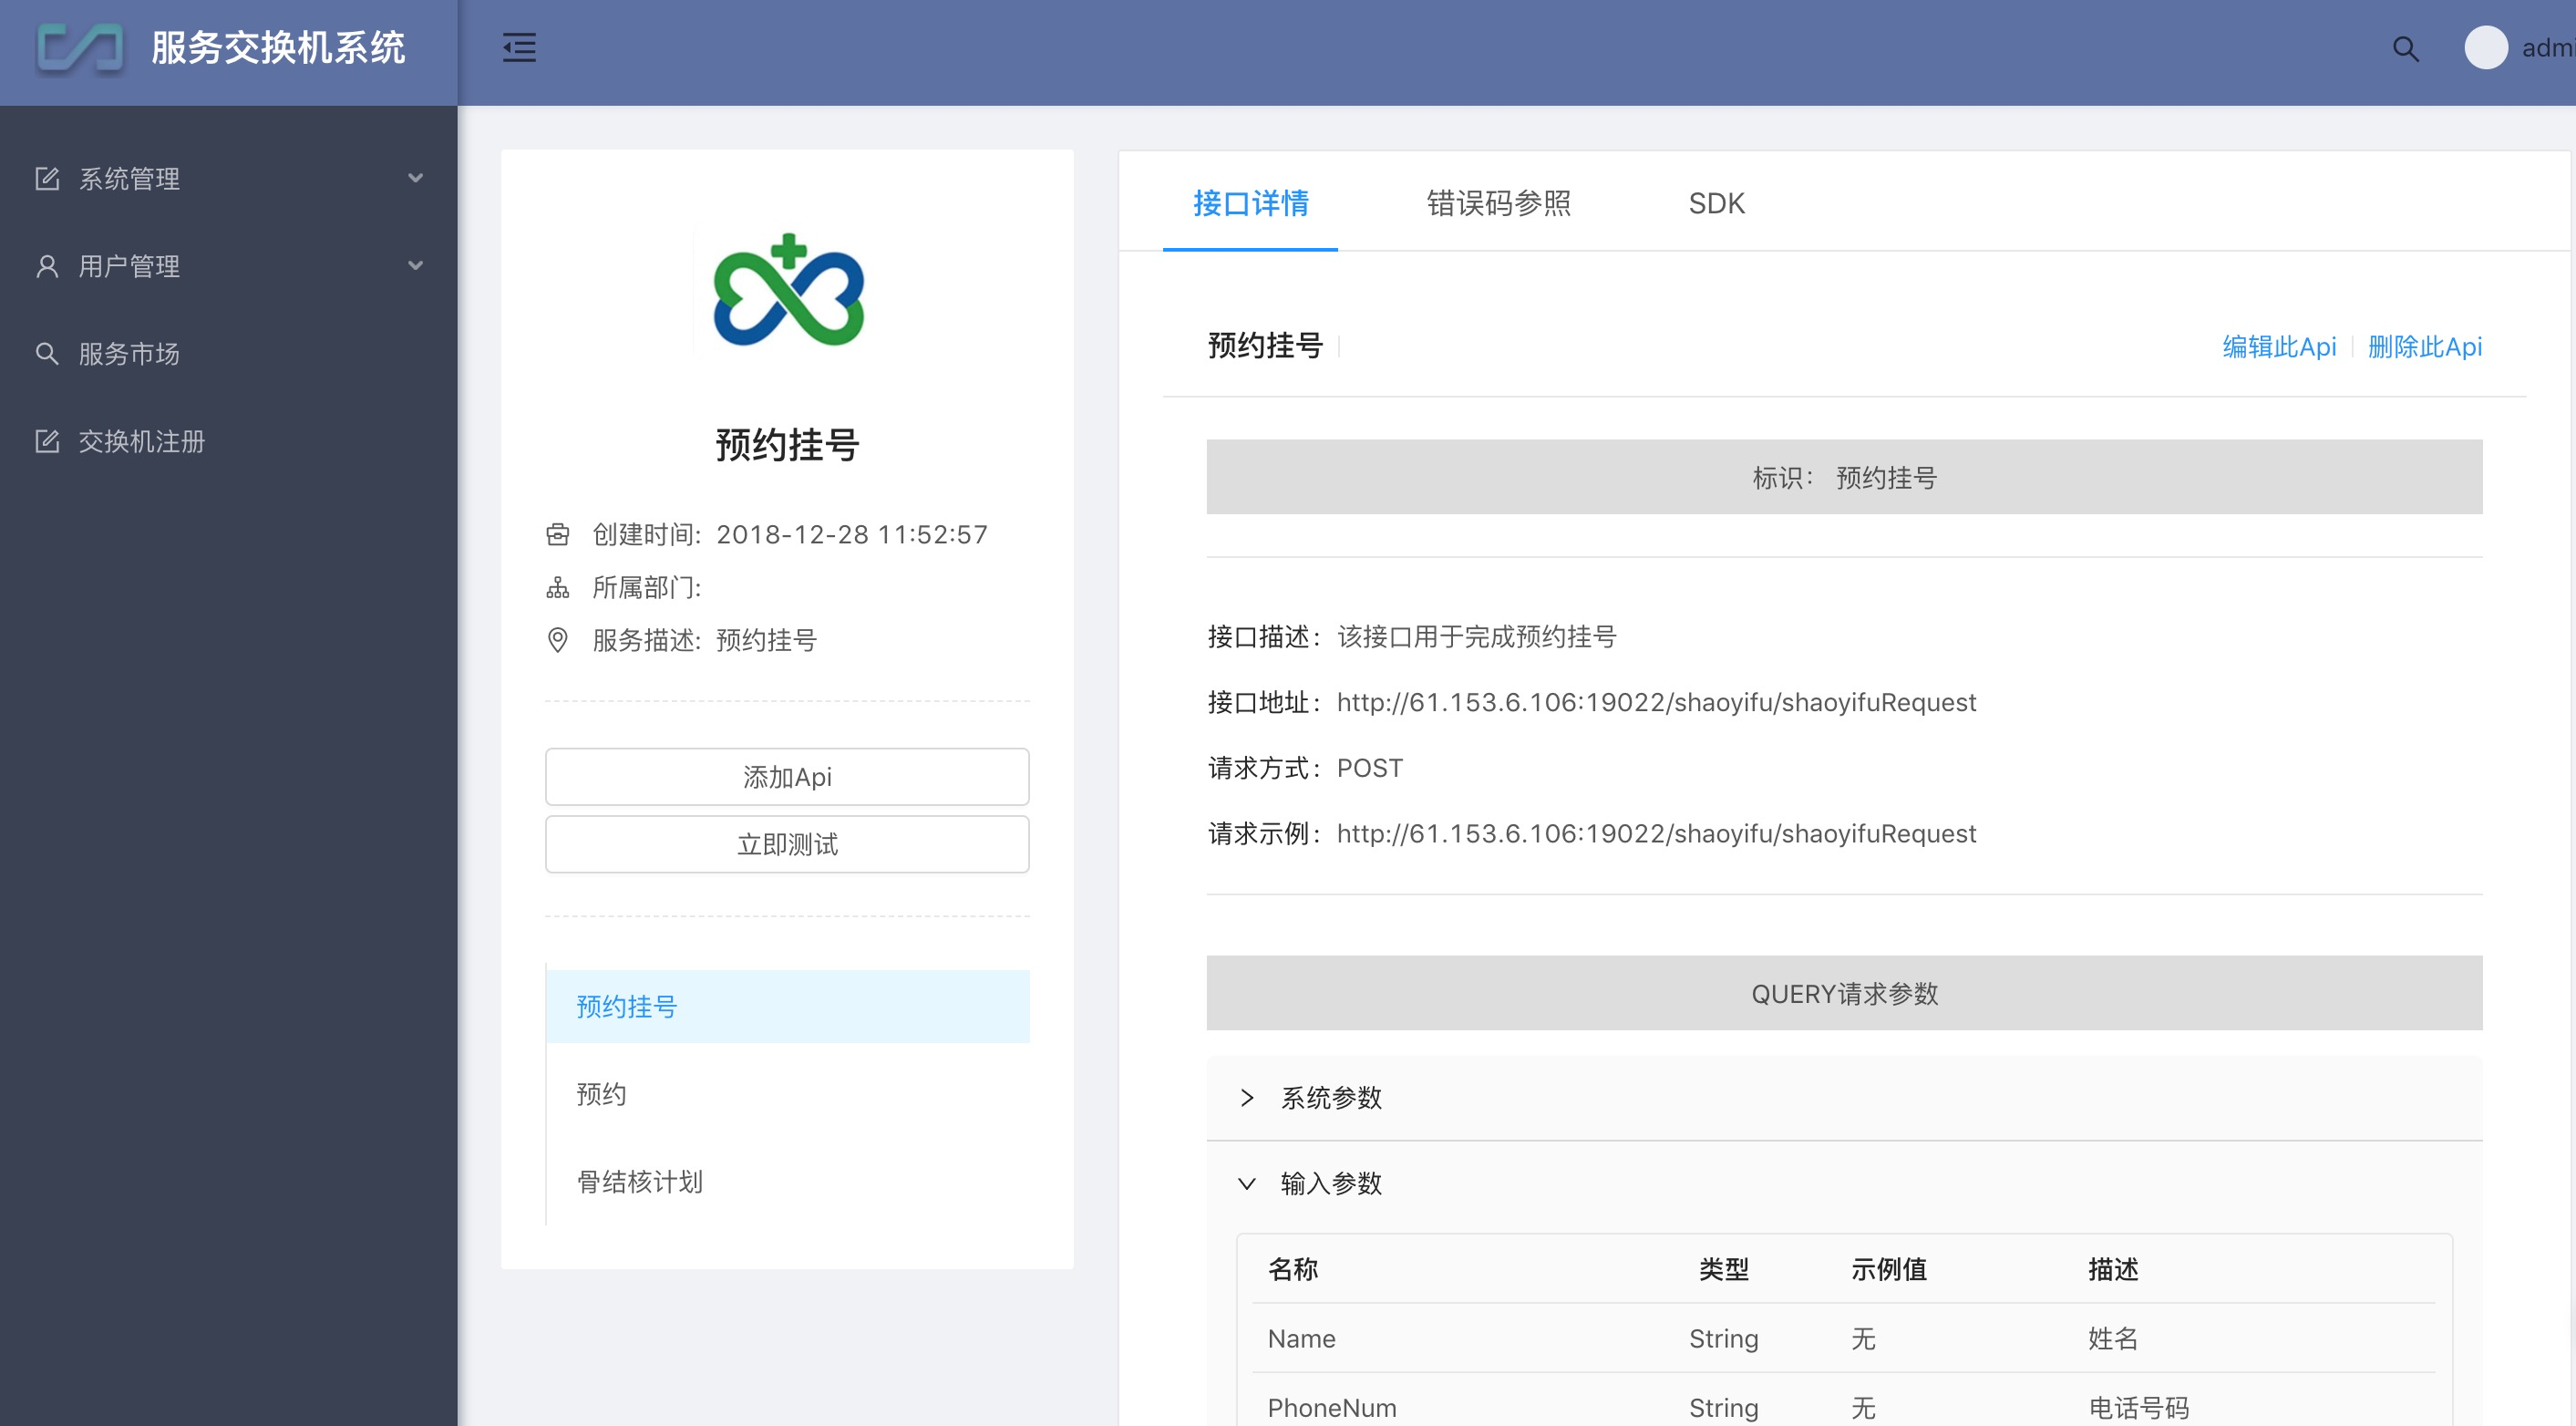
\includegraphics[width=8cm]{./images/fuwuguanli2.png}
  \label{fig:fuwuguanli2}
  }
  \caption{服务交换机管理模块}
  \label{fig:fuwuguanli}
  \end{figure}

%   \subsection{服务交换机工具模块}
%   本模块包括标准服务映射,物联网服务,服务包装等功能,其中标准服务映射是核心。
%   标准服务映射围绕在研究跨界服务集
%   成和交互过程中发现的 Web API 描述文档缺乏、描述方式不一致等导致的集成困难、难以
%   交互,以及服务使用者使用 Web API 过程中遇到的门槛较高、难以上手,需要根据自身需
%   求进行包装和定制操作,同类服务难以选择,以及 Web API 演化导致的应用失败等实际问
%   题进行了深入的研究和分析,提出了一套以服务映射为基础的自定义服务的解决方案,不但能够有效解决跨系统的 Web API 集成问题,而且提出了以用
%   户为中心的 Web API 的使用方式,能够大大简化和改善用户使用 Web API 的流程和体验,
% 还能够避免 Web API 演化带来的应用失败的问题。
%   \begin{figure}[htbp]
%     \subfloat[标准服务映射]{
%       \centering
%       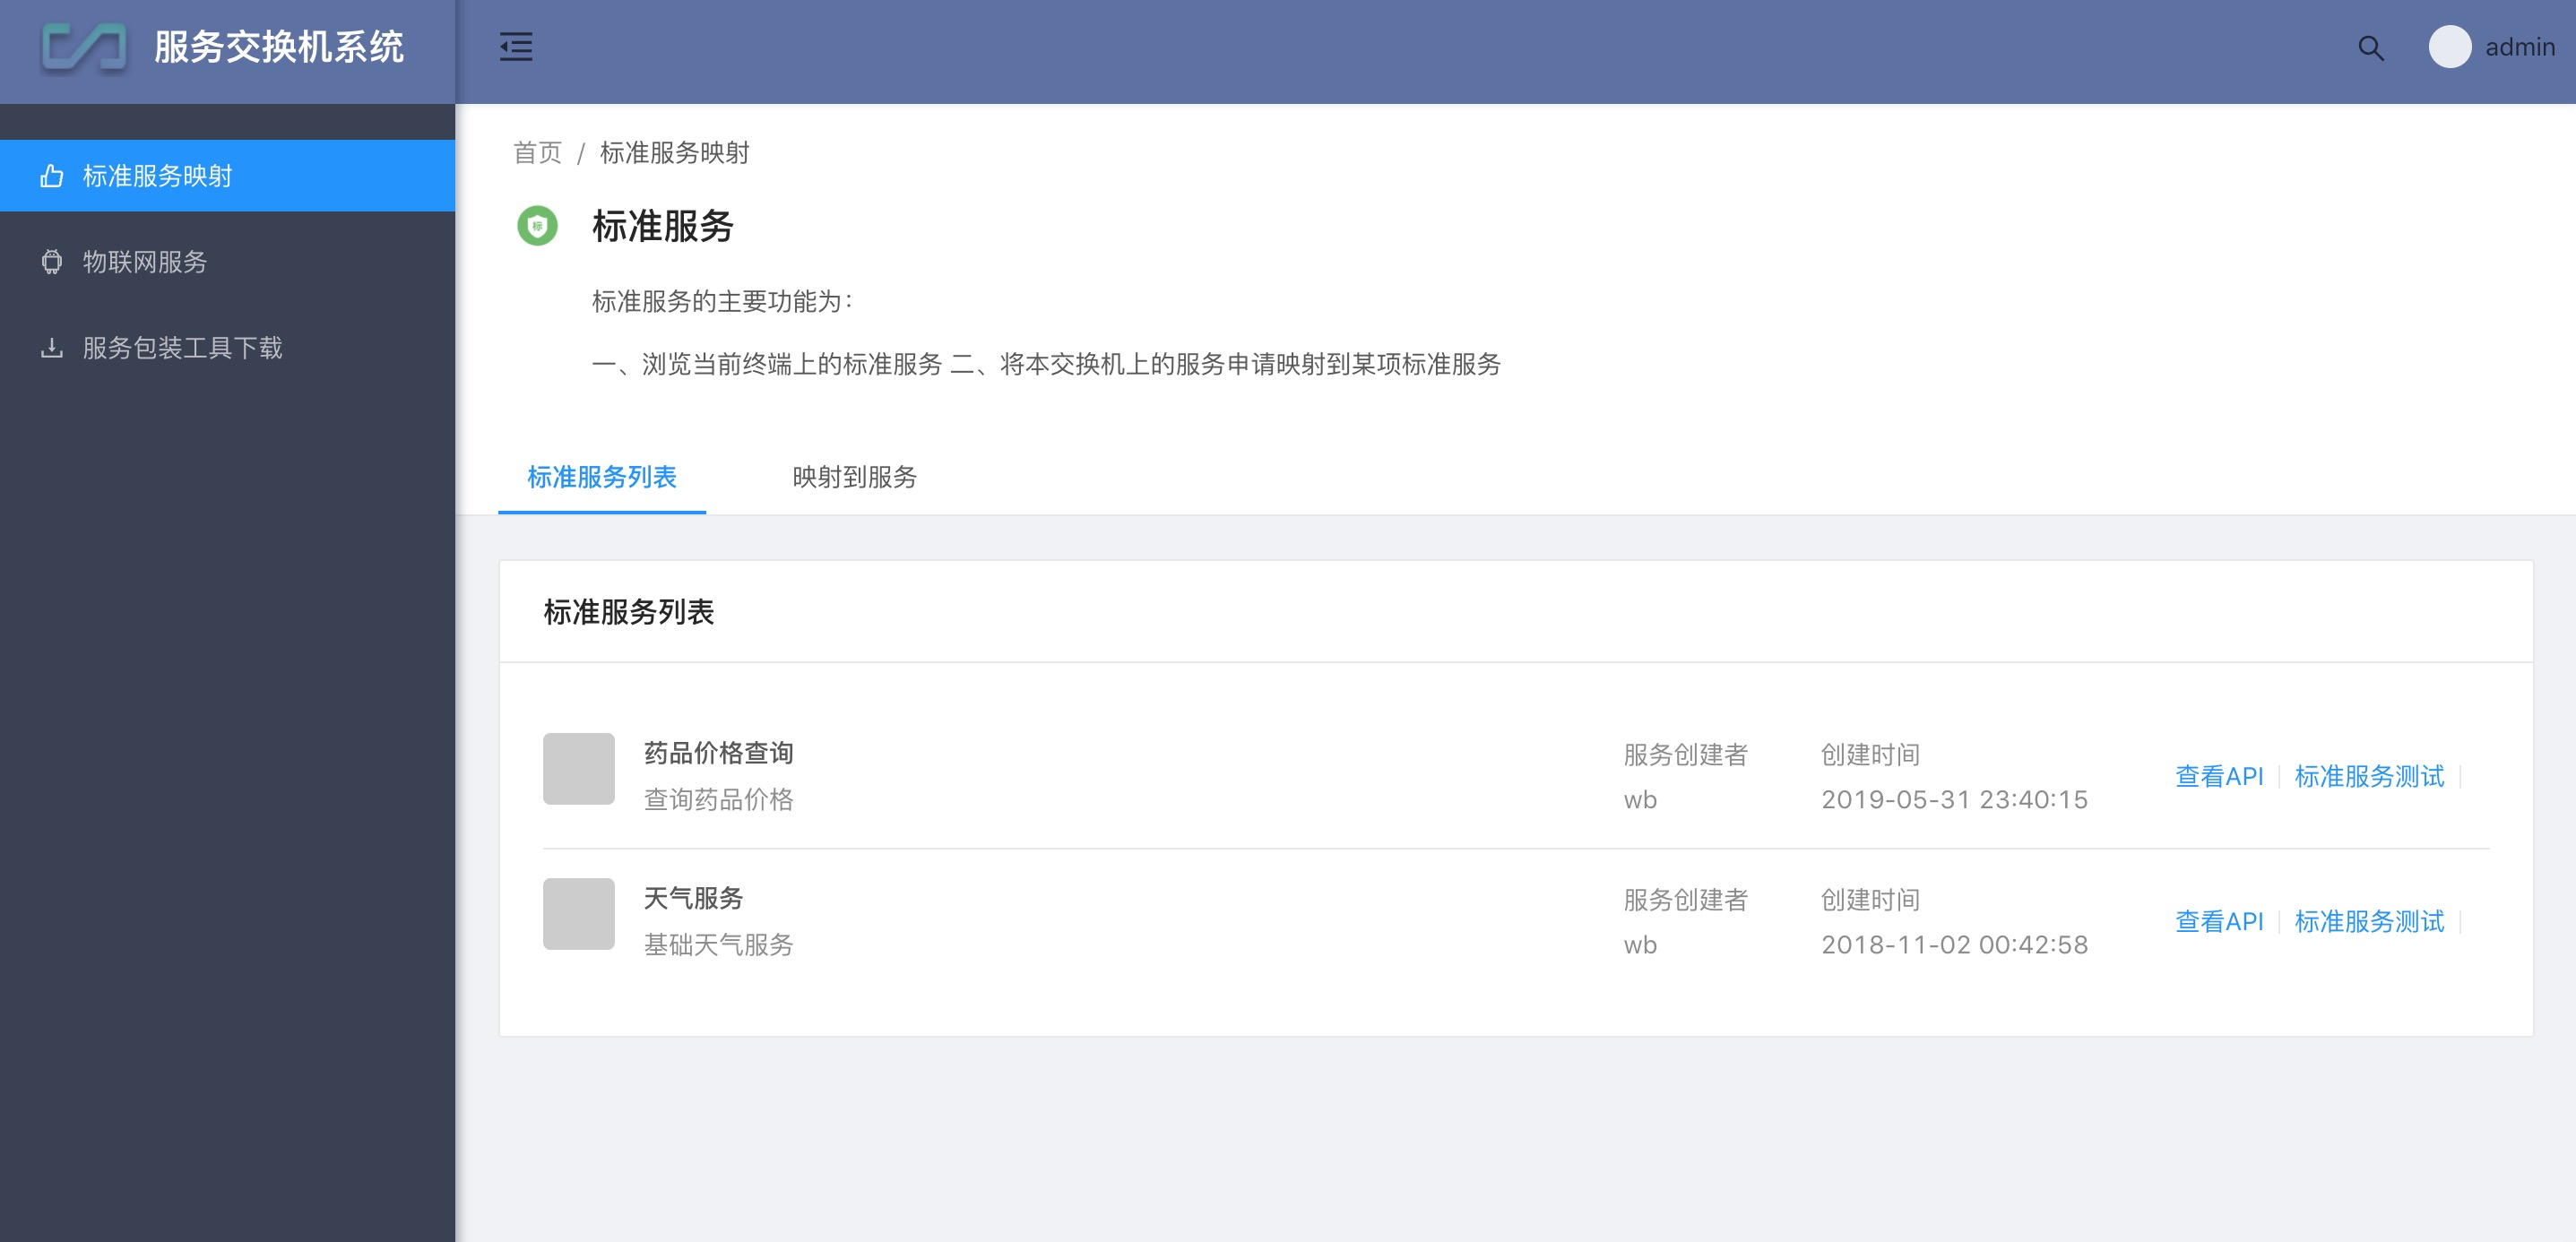
\includegraphics[width=8cm]{./images/fuwugongju1.png}
%       \label{fig:fuwugongju1}
%     }
%     \subfloat[物联网服务]{
%       \centering
%     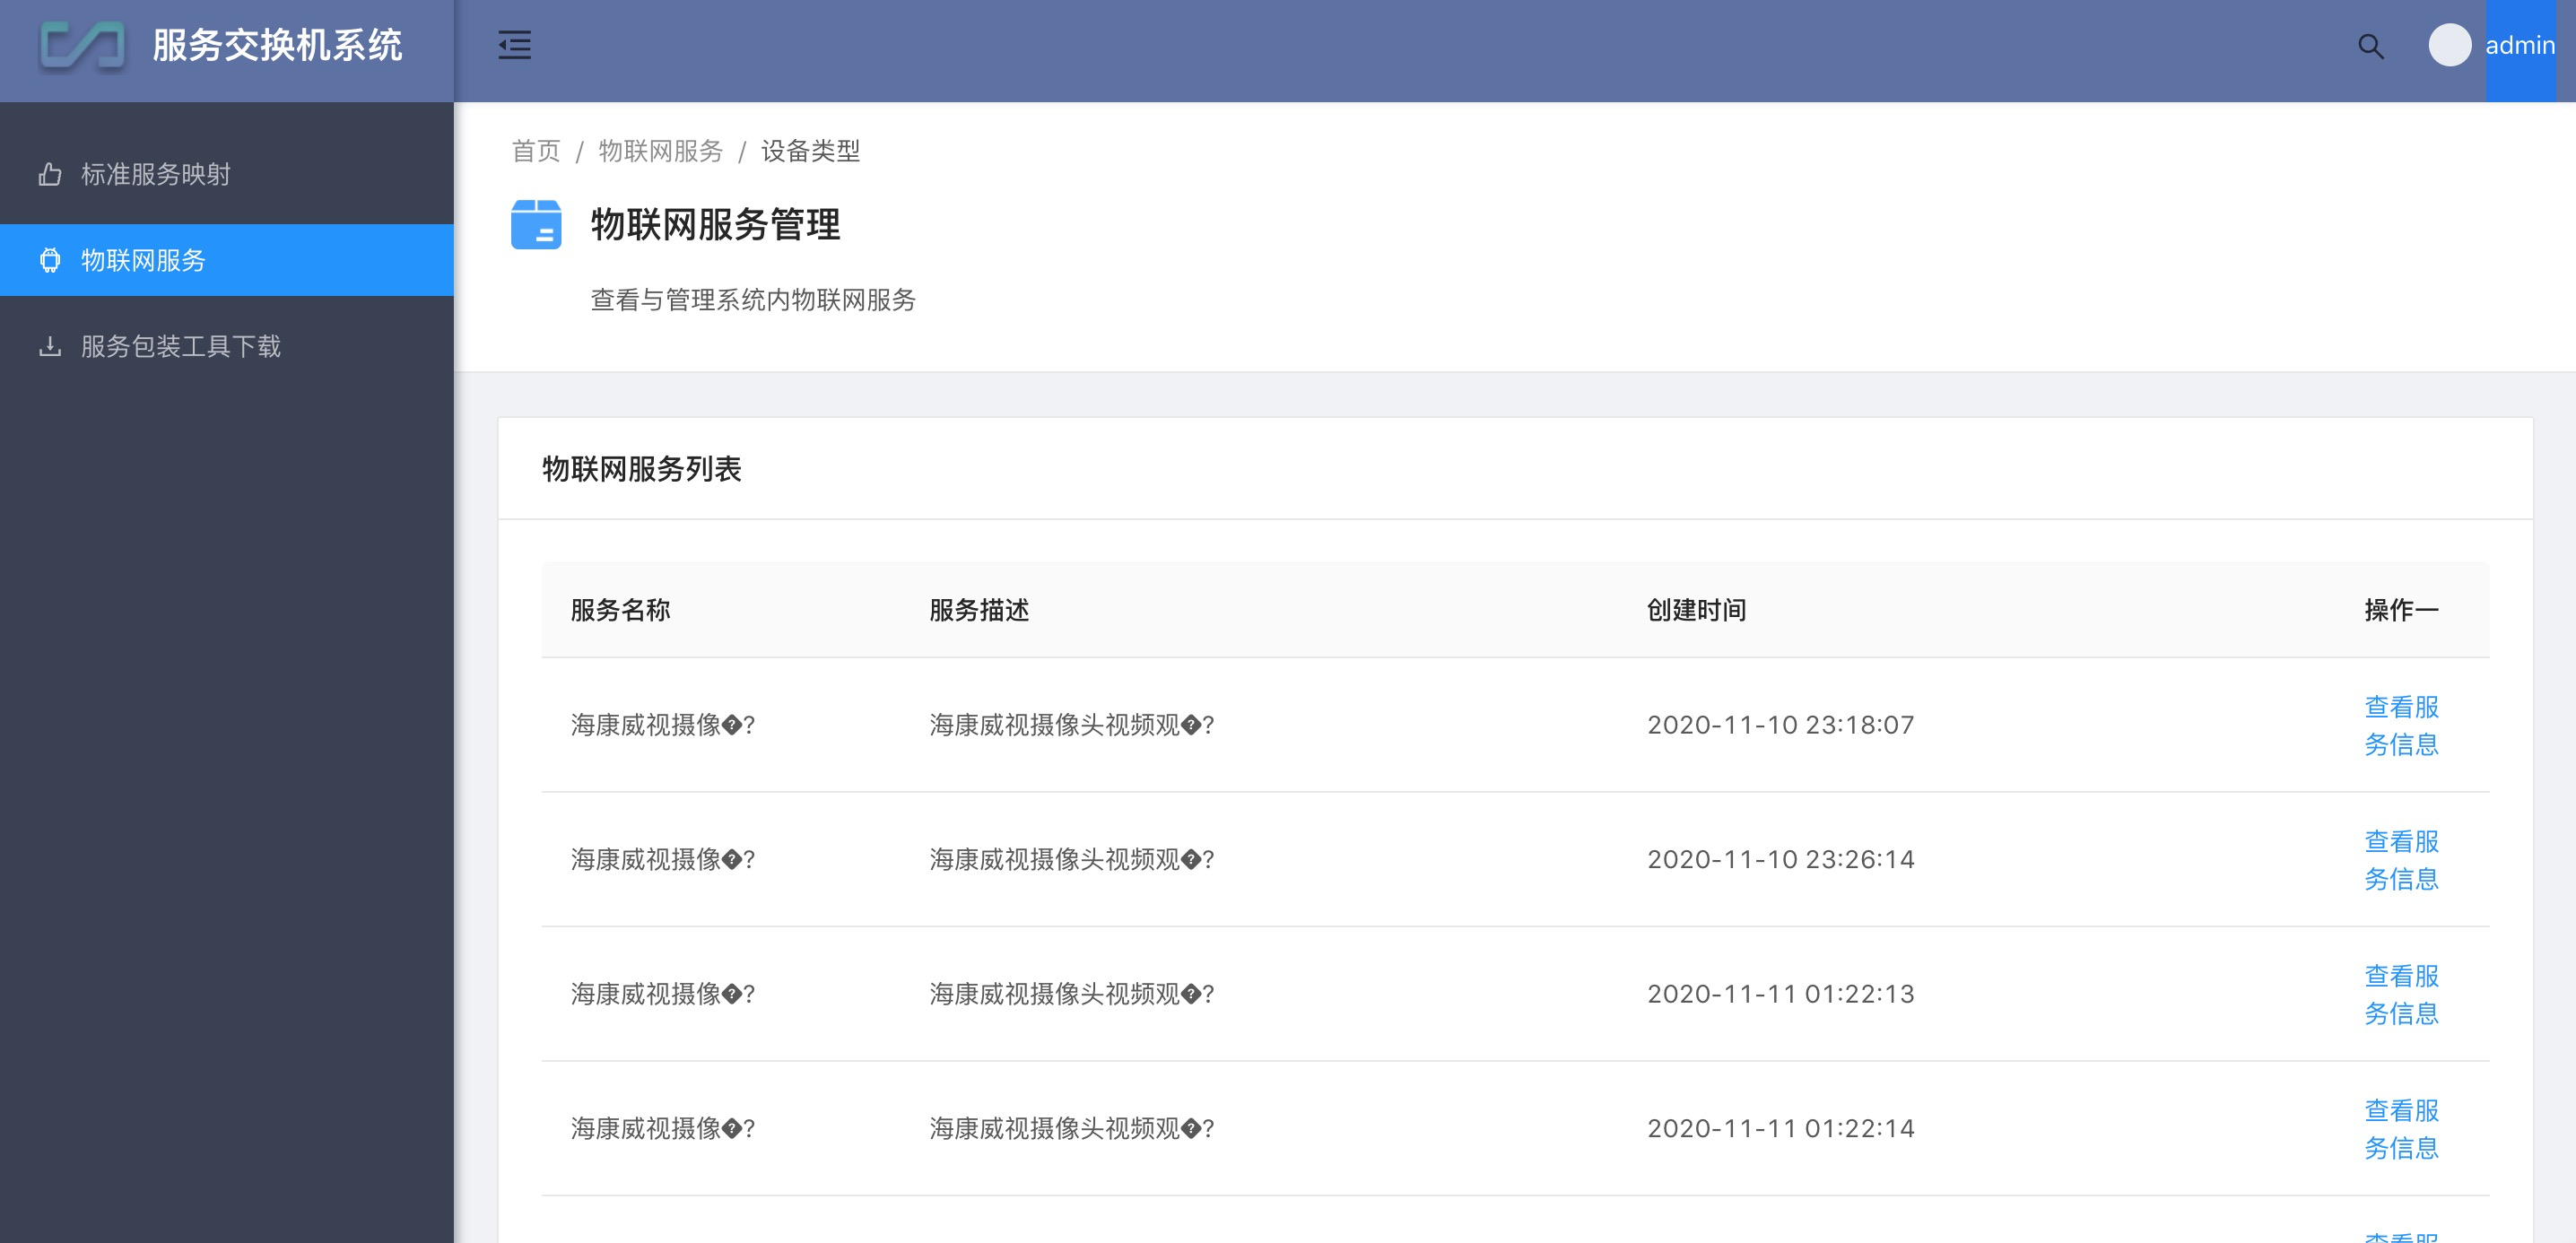
\includegraphics[width=8cm]{./images/fuwugongju2.png}
%     \label{fig:fuwugongju2}
%     }
%     \caption{服务交换机工具模块}
%     \label{fig:fuwugongju}
%     \end{figure}
\section{本章小结}
本章首先介绍了跨界服务网络的系统架构以及其核心组件服务交换机和服务路由器,之后介绍了智能服务调用引擎的系统架构,
最后展示了课题组目前跨界服务网络平台的原型系统JTangYdrail。
